%%
%% This is file `tikzposter-example.tex',
%% generated with the docstrip utility.
%%
%% The original source files were:
%%
%% tikzposter.dtx  (with options: `tikzposter-example.tex')
%% 
%% This is a generated file.
%% 
%% Copyright (C) 2014 by Pascal Richter, Elena Botoeva, Richard Barnard, and Dirk Surmann
%% 
%% This file may be distributed and/or modified under the
%% conditions of the LaTeX Project Public License, either
%% version 2.0 of this license or (at your option) any later
%% version. The latest version of this license is in:
%% 
%% http://www.latex-project.org/lppl.txt
%% 
%% and version 2.0 or later is part of all distributions of
%% LaTeX version 2013/12/01 or later.
%% 

 \documentclass[25pt, a0paper, portrait, margin=0mm, innermargin=15mm,
     blockverticalspace=10mm, colspace=10mm, subcolspace=8mm]{tikzposter} %Default values for poster format options.


 % Commands
 \newcommand{\bs}{\textbackslash}   % backslash
 \newcommand{\cmd}[1]{{\bf \color{red}#1}}   % highlights command

\usepackage[utf8]{inputenc}
\usepackage{multicol}

 % Title, Author, Institute
 \title{CP based Sequence Mining on the cloud using spark}
 \author{Cyril de Vogelaere, Pierre Schaus, John O.R. Aoga}
 \institute{UCL - Université catholique de Louvain}

 % -- PREDEFINED THEMES ---------------------- %
 % Choose LAYOUT:  Default, Basic, Rays, Simple, Envelope, Wave, Board, Autumn, Desert,
%\usetheme{Wave}
%\useblockstyle{Default}
\usetheme{Autumn}
\usecolorstyle[colorPalette=BrownBlueOrange]{Germany}

\graphicspath{ {./img/} }

\begin{document}

\maketitle

\block[roundedcorners=40]{Objectif :}{
	\Large
	The objective of this master thesis is to develop a \textbf{scalable} and \textbf{efficient} CP based implementation of the prefix-span algorithm using Spark, and to release the developed algorithm for the benefit of the Spark community.
}

\begin{columns}%blocks will be placed into columns

\column{.70}

	\block[roundedcorners=40]{Research based upon :}{
		\begin{itemize}
			\item \textbf{PPIC} : \newline
				Developed by John O.R. Aoga during his master thesis, this algorithm offer record breaking performances, \textbf{outperforming specialized system through the use of a generic constraint solver}. The main two improvement being the pre-computation of the positions at which a symbol becomes unsupported by a sequence and the usage of a backtracking-aware data structure that allows fast incremental storing and restoring of the projected database.
				
			\item \textbf{Spark} : \\
				\begin{minipage}{.45\textwidth}
				An \textbf{open source cluster computing framework} providing programmers with an application programming interface centered on a data structure called the \textbf{resilient distributed dataset} (RDD), a read-only multiset of data items distributed over a cluster of machines, that is maintained in a fault-tolerant way.\newline
				
				\textbf{Spark also disposes of a machine learning library}, which already provides an efficient prefix-span based implementation (\textbf{BFS}). The idea is thus to build upon that implementation, to develop a, more efficient, CP based solution. 
				\end{minipage}%
				\begin{minipage}{.2\textwidth}
					\begin{center}
					\begin{tikzfigure}[Spark's architecture]
						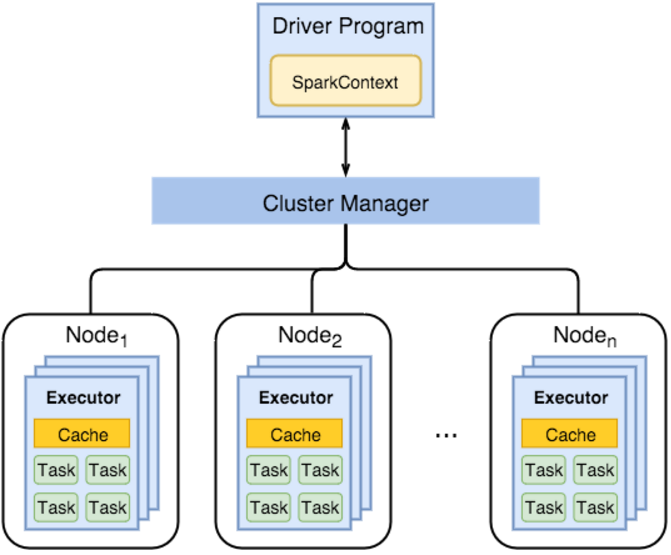
\includegraphics[scale=0.5]{architectureSpark.png}
					\end{tikzfigure}
					\end{center}
				\end{minipage}%
				
		\end{itemize}
	}
	
\column{.30}
	
	\block[roundedcorners=40]{Prefix-span algorithm:}{
		PPIC is based on the \textbf{prefix-span algorithm}. It works by analysing the current sequence to find frequent items, then it extends the current prefix and repeat the process, backtracking when necessary (\textbf{DFS}), thus generating all postfixes incrementally.
		
		\begin{tikzfigure}[Prefix-span, an easy example]
			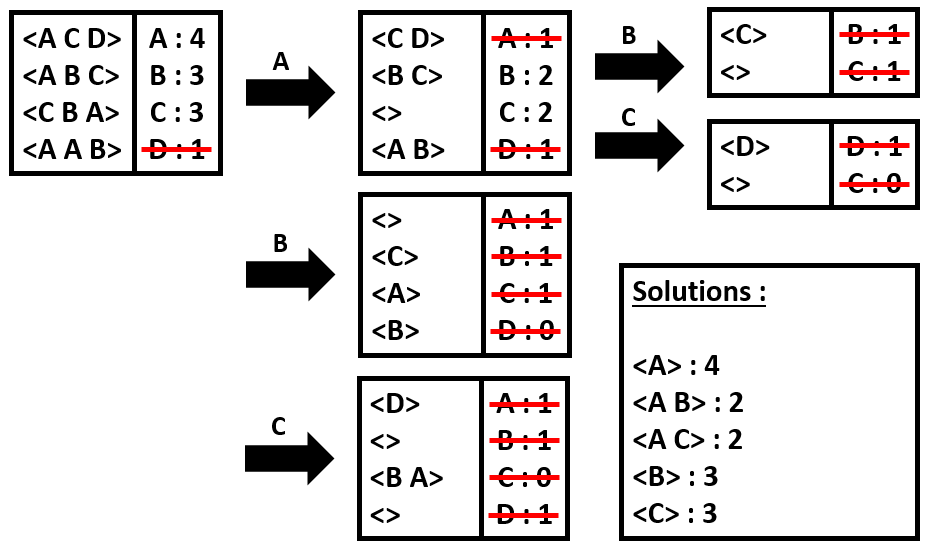
\includegraphics[scale=0.54]{prefixSpanExample.png}
		\end{tikzfigure}
	}
	
\end{columns}

\begin{columns}%blocks will be placed into columns

\column{.50}

	\block[roundedcorners=40]{PPIC vs Specialized solvers :}{
		%\center
		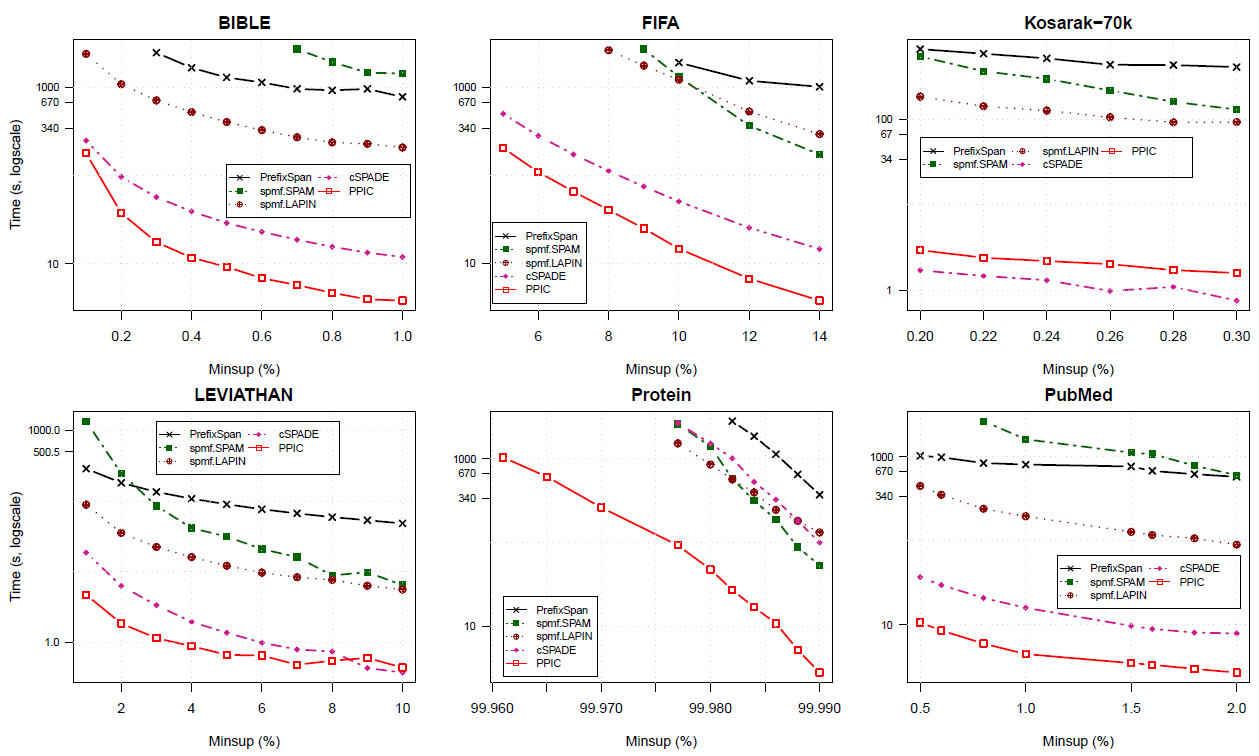
\includegraphics[scale=0.84]{PPICvsSpecialised.png}
	}
	
\column{.50}
	
	\block[roundedcorners=40]{PPIC vs Spark's original implementation :}{
		\Large
		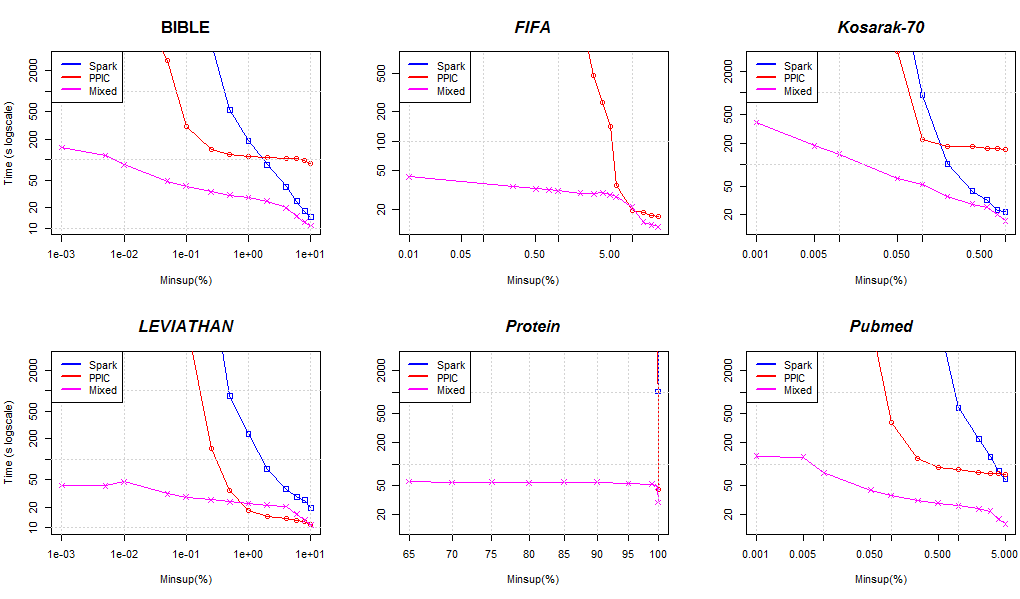
\includegraphics[scale=1.06]{OriginalPPICvsOriginalSpark.png}
	}
\end{columns}

\begin{columns}%blocks will be placed into columns

\column{.45}

	\block[roundedcorners=40]{Flaws of the original algorithms :}{
		\begin{itemize}
			\item \textbf{PPIC} :
			\begin{itemize}
				\item The algorithm is not scalable
				\item Although PPIC is ridiculously fast, the \textbf{pre-computation} needed before the algorithm can be run are extremely slow and/or \textbf{consume so much memory that the algorithm crashes}.
			\end{itemize}
				
			\item \textbf{Spark} :
			\begin{itemize}
				\item The algorithm \textbf{searches for permutations even if there are none}, which is a \textbf{huge waste of time and space}.
				\item While searching for permutations, the partialStarts array can grow exponentially large depending on the problem, leading to memory issues and massive slowdowns.
			\end{itemize}
				
				
		\end{itemize}
	}
	
	\block[roundedcorners=40]{Merging the two algorithms, how it solves our problems :}{
		\begin{itemize}
				\item We \textbf{split the search tree using Spark's algorithm} then switch to \textbf{PPIC during the local execution}. This way, the preprocessing matrices are kept to manageable sizes, effectively speeding up the whole algorithm, while making PPIC scalable.
				\item We can modify Spark's original algorithm so it \textbf{doesn't search for permutations uselessly}, as shown in the no permutation algorithm (see graph on the right). We can also switch earlier to a local execution, reducing the cost of transferring the  huge partialStart array around.
			\end{itemize}
	}
	
\column{.55}
	
	\block[roundedcorners=40]{Performance comparison of various merged algorithm :}{
		\Large
		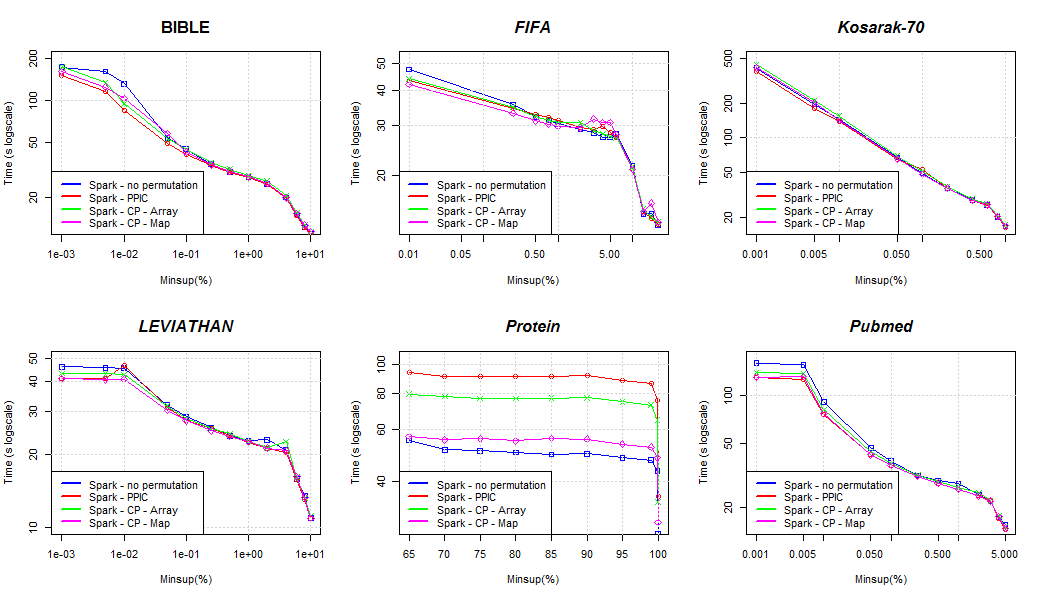
\includegraphics[scale=1.14]{PerfomComp.png}
	}
	
	\block[roundedcorners=40]{What's left to do :}{
		\begin{multicols}{2}
			\begin{itemize}
			\item Finish tests on datasets with permutations !
			\item Perform scalability tests !
			\item Start working on the paper
			\item Implement an early local switch.
			\item Propose the end result to the Spark community.
			\end{itemize}
		\end{multicols}
	}
\end{columns}

\end{document}
\endinput
%%
%% End of file `tikzposter-example.tex'.
